\documentclass{beamer}

\usetheme{McMaster}
\usepackage{math}

%===Specific for this talk===%
\usepackage{algorithm,algorithmicx,algpseudocode}
\newtheorem{proposition}{Proposition}
\DeclareMathOperator{\Span}{span}
\DeclareMathOperator{\argmin}{argmin}
\DeclareMathOperator{\adj}{adj}
\usepackage{tikz, pgfplots}
\usepackage{tikz-3dplot}
\usetikzlibrary{decorations.pathreplacing,positioning,calc,intersections,3d,shapes.geometric,shapes,chains,math,fit,backgrounds}

\title{Symmetrized cells in adaptive optimized Schwarz}
\author{Conor McCoid}
\institute{McMaster University}
\date{June 24th, 2025}

\begin{document}

\maketitle

\section{Domain decomposition}

\begin{frame}
\frametitle{What is domain decomposition?}

\begin{columns}
	\begin{column}{0.5\textwidth}
		Domain decomposition splits large complicated domains into smaller, easier subdomains.
		The problem is solved on each subdomain, information is passed to other subdomains, then solved on subdomains again, etc., creating an iterative method.
	\end{column}
	\begin{column}{0.5\textwidth}
		\begin{figure}
			\centering
			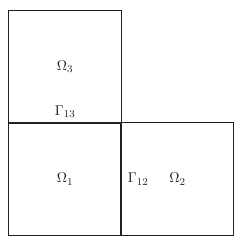
\includegraphics[width=\textwidth]{FIG/Saad_Lshape_domains.png}
			\caption{Example taken from ``Iterative Methods for Sparse Linear Systems'', by Yousef Saad}
		\end{figure}
	\end{column}
\end{columns}
\end{frame}

\begin{frame}
\frametitle{Discretization of the example}

\begin{columns}
	\begin{column}{0.5\textwidth}
		Now that we have our continuous domain decomposition, we need to discretize the problem and split up the unknowns.
	\end{column}
	\begin{column}{0.5\textwidth}
		\begin{figure}
			\centering
			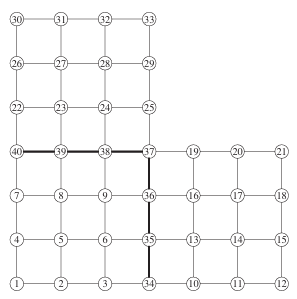
\includegraphics[width=\textwidth]{FIG/Saad_Lshape_nodes.png}
			\caption{Nodes for example}
		\end{figure}
	\end{column}
\end{columns}
\end{frame}

\begin{frame}
\frametitle{Matrix of the example}

\begin{columns}
	\begin{column}{0.5\textwidth}
		This discretization, with this ordering for the nodes, comes with a matrix, with one row and one column per node.
		The dashed lines show how the domain decomposition splits up the unknowns.
	\end{column}
	\begin{column}{0.5\textwidth}
		\begin{figure}
			\centering
			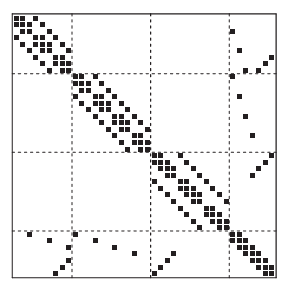
\includegraphics[width=\textwidth]{FIG/Saad_Lshape_matrix.png}
			\caption{Matrix for example based on nodes}
		\end{figure}
	\end{column}
\end{columns}
\end{frame}

\begin{frame}
\frametitle{More complicated example}
\begin{columns}
	\begin{column}{0.5\textwidth}
		\begin{figure}
			\centering
			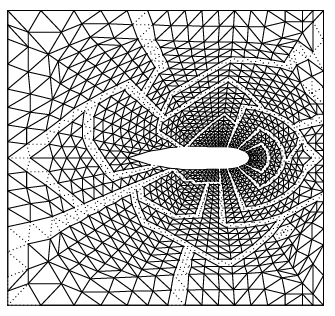
\includegraphics[width=\textwidth]{FIG/Saad_airfoil.png}
			\caption{Also from Saad's ``Iterative Methods''}
		\end{figure}
	\end{column}
	\begin{column}{0.5\textwidth}
		\begin{figure}
			\centering
			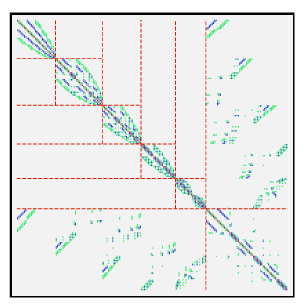
\includegraphics[width=\textwidth]{FIG/Saad_cover.png}
			\caption{Possible matrix for example}
		\end{figure}
	\end{column}
\end{columns}
\end{frame}

\begin{frame}
\frametitle{A general form of the matrix}

In this talk, let us consider matrices that can take the form
\begin{equation} \label{eq: lin sys}
	\begin{bmatrix}
		A_{11} & & & & A_{1 \Gamma} \\
		& A_{22} & & & A_{2 \Gamma} \\
		& & \ddots & & \vdots \\
		& & & A_{nn} & A_{n \Gamma} \\
		A_{\Gamma 1} & A_{\Gamma 2} & \dots & A_{\Gamma n} & A_{\Gamma \Gamma}
	\end{bmatrix}
	\begin{bmatrix} \vec{u}_1 \\ \vec{u}_2 \\ \vdots \\ \vec{u}_n \\ \vec{u}_\Gamma \end{bmatrix}
	=
	\begin{bmatrix} \vec{f}_1 \\ \vec{f}_2 \\ \vdots \\ \vec{f}_n \\ \vec{f}_\Gamma \end{bmatrix},
\end{equation}
where $A_{ii}$ are square.
This system represents $n$ subdomains connected through a global interface represented by $\Gamma$.

\end{frame}

\begin{frame}
\frametitle{The subproblems}

Each subdomain now has its own subproblem:
\begin{equation} \label{eq: subproblem}
	\begin{bmatrix}
		A_{ii} & A_{i \Gamma} \\
		A_{\Gamma i} & A_{\Gamma \Gamma} + S_i
	\end{bmatrix}
	\begin{bmatrix} \vec{u}_i \\ \vec{u}_\Gamma \end{bmatrix}
	=
	\begin{bmatrix} \vec{f}_i \\ \tilde{\vec{f}}_i \end{bmatrix},
\end{equation}
where $\tilde{\vec{f}}_i$ is some modification of $\vec{f}_\Gamma$,
and $S_i$ is some global transmission matrix.

We see that the variables associated with the global interface $\Gamma$ appear in all subproblems.
The global transmission matrix $S_i$ dictates how these many copies communicate with one another.
\end{frame}

\begin{frame}
\frametitle{How to choose $S_i$ and $\tilde{\vec{f}}_i$}

There are perfect choices of $S_i$ and $\tilde{\vec{f}}_i$ such that each subproblem gives the exact solution to the global problem on its respective subdomain.
However, these perfect choices are expensive to compute.

Instead, the standard procedure is to make \textit{a priori} choices that give convergent iterative methods.
These appear as:
\begin{equation} \label{eq: iterative sub}
	\begin{bmatrix}
		A_{ii} & A_{i \Gamma} \\
		A_{\Gamma i} & A_{\Gamma \Gamma} + S_i
	\end{bmatrix}
	\begin{bmatrix} \vec{u}_i^{(k+1)} \\ \vec{u}_{\Gamma i}^{(k+1)} \end{bmatrix}
	=
	\begin{bmatrix} \vec{f}_i \\ \vec{f}_\Gamma \end{bmatrix}
	+ \sum_{j \neq i}
	\begin{bmatrix} ~ \\ -A_{\Gamma j} & T_j \end{bmatrix}
	\begin{bmatrix} \vec{u}_j^{(k)} \\ \vec{u}_{\Gamma j}^{(k)} \end{bmatrix},
\end{equation}
where
\begin{equation} \label{eq: local to global transmission}
	S_i = \sum_{j \neq i} T_j.
\end{equation}
\end{frame}

\begin{frame}
\frametitle{Choices for $T_j$}

The local transmission matrices $T_j$ can represent boundary conditions between the subdomains.
Some common options:
\begin{itemize}
\item Dirichlet, setting the interface variables on subdomain 2 equal to those found on subdomain 1
\item Neumann, setting the derivatives to be the same
\item Optimized, setting Robin boundary conditions to be the same, using a Robin parameter that optimizes convergence rates
\end{itemize}

In this talk, there won't be an \textit{a priori} choice.
The transmission matrices will adapt to the iterative method.

\end{frame}

\section{Symmetrized cells}

\begin{frame}
\frametitle{What is a symmetrized cell?}

\begin{columns}
	\begin{column}{0.5\textwidth}
For each subdomain, take a copy of it and stitch it together along their shared interface.
This pair is now perfectly symmetric, and one subproblem describes both copies.
	\end{column}

\tdplotsetmaincoords{60}{110}
\def\SplitAngle{120}
\def\AngleSplit{300}
	\begin{column}{0.5\textwidth}
\begin{figure}
	\begin{tikzpicture}[tdplot_main_coords]
		\fill[left color=blue!50] (180:1 and 1) arc (180:\AngleSplit:1 and 1) -- ++(0,0,2) arc (\AngleSplit:180:1 and 1) -- cycle;
		\fill[left color=blue!50] (1,0,0) arc (360:\AngleSplit:1 and 1) -- ++(0,0,2) arc (\AngleSplit:360:1 and 1) -- cycle;
		\foreach \x in {-2,...,2} {
			\draw[gray, thin] (\x,0,-1) -- (\x,0,3);
		}
		\foreach \z in {-1,...,3} {
			\draw[gray, thin] (-2,0,\z) -- (2,0,\z);
		}
		\fill[right color=red!10] (\SplitAngle:1 and 1) arc (\SplitAngle:180:1 and 1) -- ++(0,0,2) arc (180:\SplitAngle:1 and 1) -- cycle;
		\fill[right color=red!10] (1,0,0) arc (0:\SplitAngle:1 and 1) -- ++(0,0,2) arc (\SplitAngle:0:1 and 1) -- cycle;
	\end{tikzpicture}
	\caption{A symmetrized square domain with interfaces on two opposing edges}
\end{figure}
	\end{column}
\end{columns}
\end{frame}

\begin{frame}
\frametitle{Algebra of a symmetrized cell}

The equation for the unknowns on a symmetrized cell is:
\begin{equation} \label{eq: sym cell}
	\begin{bmatrix}
		A_{ii} & A_{i \Gamma} \\
		A_{\Gamma i} & A_{\Gamma \Gamma} & A_{\Gamma i} \\
		& A_{i \Gamma} & A_{ii}
	\end{bmatrix}
	\begin{bmatrix} \hat{\vec{u}}_i \\ \hat{\vec{u}}_\Gamma \\ \hat{\vec{u}}_i \end{bmatrix}
	=
	\begin{bmatrix} \vec{f}_i \\ \hat{\vec{f}}_i \\ \vec{f}_i \end{bmatrix}.
\end{equation}
The solution on this cell does not correspond to the solution of the global problem, but it may serve as a good initial guess.
\end{frame}

\begin{frame}
\frametitle{Subproblems of the cell}

The iterative process of solving the equation on the cell is then solving repeatedly the equation:
\begin{equation} \label{eq: sym cells}
	\begin{bmatrix}
		A_{ii} & A_{i \Gamma} \\
		A_{\Gamma i} & A_{\Gamma \Gamma} + T_i^{(k+1)}
	\end{bmatrix}
	\begin{bmatrix} \vec{u}_i^{(k+1)} \\ \vec{u}_{\Gamma i}^{(k+1)} \end{bmatrix}
	=
	\begin{bmatrix} \vec{f}_i \\ \hat{\vec{f}}_i \end{bmatrix}
	+
	\begin{bmatrix} ~ \\ -A_{\Gamma i} & T_i^{(k)} \end{bmatrix}
	\begin{bmatrix} \vec{u}_i^{(k)} \\ \vec{u}_{\Gamma i}^{(k)} \end{bmatrix}.
\end{equation}
It is often better to present this in a corrector version that acts only on the differences between successive iterates, $\vec{d}_i^{(k+1)} = \vec{u}_i^{(k+1)} - \vec{u}_i^{(k)}$:
\begin{equation} \label{eq: sym cells AOSM}
	\begin{bmatrix}
		A_{ii} & A_{i \Gamma} \\
		A_{\Gamma i} & A_{\Gamma \Gamma} + T_i^{(k+1)}
	\end{bmatrix}
	\begin{bmatrix} \vec{d}_i^{(k+1)} \\ \vec{d}_{\Gamma i}^{(k+1)} \end{bmatrix}
	=
	\begin{bmatrix} ~ \\ -A_{\Gamma i} & T_i^{(k)} \end{bmatrix}
	\begin{bmatrix} \vec{d}_i^{(k)} \\ \vec{d}_{\Gamma i}^{(k)} \end{bmatrix}.
\end{equation}
\end{frame}

\begin{frame}
\frametitle{Krylov subspace in the cell}

We can use techniques from static condensation to reduce the form of this system to acting only on the global interface:
\begin{equation}
	\vec{d}_{\Gamma i}^{(k+1)} = \left ( \hat{A}_i + E_i^{(k+1)} \right )^{-1} E_i^{(k)} \vec{d}_{\Gamma i}^{(k)},
\end{equation}
where
\begin{equation*}
	\hat{A}_i = A_{\Gamma \Gamma} - 2 A_{\Gamma i} A_{ii}^{-1} A_{i \Gamma}, \quad E_i^{(k)} = T_i^{(k)} + A_{\Gamma i} A_{ii}^{-1} A_{i \Gamma}.
\end{equation*}

This means the vectors $\vec{d}_{\Gamma i}^{(k+1)}$ form a Krylov subspace:
\begin{equation} \label{eq: Krylov subspace}
	\vec{d}_{\Gamma i}^{(k+1)} \in \mathcal{K}_{k+1} \left ( \left ( \hat{A}_i + E_i^{(k+1)} \right )^{-1} E_i^{(k)}, \vec{d}_{\Gamma i}^{(0)} \right ).
\end{equation}
\end{frame}

\begin{frame}
\frametitle{Updates to $T_i^{(k)}$}

The most important part of the symmetrized cells is the update to the transmission matrix $T_i$.
We want an update that uses information obtained in solving equations on the cell and that reduces $E_i^{(k)}$ to zero, as this means the iterative process becomes direct.

As a first approximation, use rank one updates that give the action of $E_i^{(k)}$ in the direction $\vec{d}_{\Gamma i}^{(k)}$:
\begin{equation*}
	T_i^{(k+1)} - T_i^{(k)} := - E_i^{(k)} \frac{\vec{d}_{\Gamma i}^{(k)} \left ( \vec{d}_{\Gamma i}^{(k)} \right )^\top}{\norm{\vec{d}_{\Gamma i}^{(k)}}^2}.
\end{equation*}
\end{frame}

\begin{frame}
\frametitle{Iterative action approximation}

If the vectors $\vec{d}_{\Gamma i}^{(k)}$ aren't orthogonal, then these updates will interfere with each other.
Run these vectors through modified Gram-Schmidt to fix this issue.
	\begin{algorithmic}[1]
		\State Inputs: $\vec{d}_{\Gamma i}^{(k)}$, $E_i^{(k)} \vec{d}_{\Gamma i}^{(k)}$, all previous $\vec{d}_{\Gamma i}^{(j)}$ and $E_i^{(j)} \vec{d}_{\Gamma i}^{(j)}$
		\State Set $\vec{w}_k := \vec{d}_{\Gamma i}^{(k)}$ and $\vec{v}_k := E_i^{(k)} \vec{d}_{\Gamma i}^{(k)}$
		\For{$j=1:k-1$}
			\State $h \gets \langle \vec{d}_{\Gamma i}^{(j)}, \vec{w}_k \rangle$, $\vec{w}_k \gets \vec{w}_k - h \vec{d}_{\Gamma i}^{(j)}$
			\State $\vec{v}_k \gets \vec{v}_k - h E_i^{(j)} \vec{d}_{\Gamma i}^{(j)}$
		\EndFor
		\State Output: $\Delta T_i^{(k+1)} := -\vec{v}_k \vec{w}_k^\top$
	\end{algorithmic}
\end{frame}

\begin{frame}
\frametitle{Krylov subspace method}

Incidentally, this will give an orthonormal basis for the Krylov subspace.
There is also an indirect Galerkin condition at work, making this process essentially equivalent to the full orthogonalization method (FOM), precursor to GMRES.

To show that,
use the Woodbury matrix identity to write $\vec{d}_{\Gamma i}^{(k+1)}$ as
\begin{equation*}
	\vec{d}_{\Gamma i}^{(k+1)} = \frac{ \left ( \hat{A}_i + E_{i}^{(k)} \right )^{-1} E_{i}^{(k)} \vec{d}_{\Gamma i}^{(k)} }{ \vec{w}_k^\top \left ( I - \left ( \hat{A}_i + E_{i}^{(k)} \right )^{-1} E_{i}^{(k)} \right ) \vec{w}_k}
\end{equation*}

\end{frame}

\begin{frame}
\frametitle{Indirect Galerkin condition}

Next, consider the following Galerkin condition:
\begin{equation*}	
	\left ( I - \left ( \hat{A}_i + E_{i}^{(k)} \right )^{-1} E_{i}^{(k)}  \right ) \vec{x} - \vec{d}_{\Gamma i}^{(k)} \perp \mathcal{K}_k, \quad \vec{x} \in \mathcal{K}_k.
\end{equation*}
The solution satisfies
\begin{equation*}
	\vec{w}_k^\top \vec{x} = \frac{\vec{w}_k^\top \vec{d}_{\Gamma i}^{(k)}}{\vec{w}_k^\top \left ( I - \left ( \hat{A}_i + E_{i}^{(k)} \right )^{-1} E_{i}^{(k)} \right ) \vec{w}_k} .
\end{equation*}
Since $E_i^{(k)}$ has $\mathcal{K}_{k-1}$ in its null space, we can write $\vec{d}_{\Gamma i}^{(k+1)}$ as
\begin{equation*}
	\vec{d}_{\Gamma i}^{(k+1)} = \left ( \hat{A}_i + E_{i}^{(k)} \right )^{-1} E_{i}^{(k)} \vec{x}.
\end{equation*}

\end{frame}

\begin{frame}
\frametitle{Results of symmetrized cells}

Once the iterative process on the cell is complete, we get the following outputs:
\begin{description}
\item[excellent local transmission matrix:] the matrix $T_i$ (last to be computed) is now a very good approximation of the best possible local transmission matrix;
\item[good initial guess of the solution on the cell:] the solution $\hat{\vec{u}}_i$ is not the solution for the global problem, but it satisfies the problem locally, making it a good initial guess for the next stage.
\end{description}

\end{frame}

\begin{frame}
\frametitle{Continuous analogs}

The matrix $T_i$ approximates absorbing boundary conditions.
These conditions allow waves to pass through the boundary with no reflection.

Several methods in the continuous space have been developed to approximate ABCs:
\begin{itemize}
\item perfectly matched layers
\item one-way equations
\item change of variables
\item probing
\end{itemize}

\end{frame}

\section{Global reconstruction}

\begin{frame}
\frametitle{Putting the pieces together again}

Now that we have good transmission matrices and good initial guesses, we can solve the global problem very quickly.
Set
\begin{equation*}
	S_i = \sum_{j \neq i} T_j, \quad \vec{u}_i^{(0)} = \hat{\vec{u}}_i,
\end{equation*}
then solve
\begin{equation*}
	\begin{bmatrix}
		A_{ii} & A_{i \Gamma} \\
		A_{\Gamma i} & A_{\Gamma \Gamma} + S_i
	\end{bmatrix}
	\begin{bmatrix} \vec{u}_i^{(k+1)} \\ \vec{u}_{\Gamma i}^{(k+1)} \end{bmatrix}
	=
	\begin{bmatrix} \vec{f}_i \\ \vec{f}_\Gamma \end{bmatrix}
	+ \sum_{j \neq i}
	\begin{bmatrix} ~ \\ -A_{\Gamma j} & T_j \end{bmatrix}
	\begin{bmatrix} \vec{u}_j^{(k)} \\ \vec{u}_{\Gamma j}^{(k)} \end{bmatrix},
\end{equation*}
or a corrector version if preferred:
\begin{equation*}
	\begin{bmatrix}
		A_{ii} & A_{i \Gamma} \\
		A_{\Gamma i} & A_{\Gamma \Gamma} + S_i
	\end{bmatrix}
	\begin{bmatrix} \vec{d}_i^{(k+1)} \\ \vec{d}_{\Gamma i}^{(k+1)} \end{bmatrix}
	= \sum_{j \neq i}
	\begin{bmatrix} ~ \\ -A_{\Gamma j} & T_j \end{bmatrix}
	\begin{bmatrix} \vec{d}_j^{(k)} \\ \vec{d}_{\Gamma j}^{(k)} \end{bmatrix}.
\end{equation*}
\end{frame}

\begin{frame}
\frametitle{Condensed equation}

Using the corrector version and the same techniques from static condensation, the iteration can be represented acting solely on the global interface:
\begin{equation*}
	\left ( \hat{A} + \sum_{j \neq i} E_j \right ) \vec{d}_{\Gamma i}^{(k+1)} = \sum_{j \neq i} E_j \vec{d}_{\Gamma j}^{(k)},
\end{equation*}
where
\begin{equation*}
	\hat{A} = A_{\Gamma \Gamma} - \sum_{i=1}^n A_{\Gamma i} A_{ii}^{-1} A_{i \Gamma}, \quad E_j = T_j + A_{\Gamma j} A_{jj}^{-1} A_{j \Gamma}.
\end{equation*}

\end{frame}

\begin{frame}
\frametitle{Convergence rate}

This means the convergence of the global reconstruction is defined by
\begin{equation*}
	\begin{bmatrix} \vdots \\ \vec{d}_{\Gamma i}^{(k+1)} \\ \vdots \end{bmatrix}
	=
	\begin{bmatrix} \ddots \\ & \hat{A} + \sum_{j \neq i} E_j \\ & & \ddots \end{bmatrix}^{-1}
	\begin{bmatrix} & E_2 & E_3 & \dots \\ E_1 & & E_3 & \dots \\ E_1 & E_2 \\ \vdots & \vdots & & \ddots \end{bmatrix}
	\begin{bmatrix} \vdots \\ \vec{d}_{\Gamma i}^{(k)} \\ \vdots \end{bmatrix}.
\end{equation*}
The spectral radius of the matrix in this equation then dictates the convergence rate.
After the symmetrized cells iterations, this spectral radius should be small, but more analysis is needed to confirm this in general.

\end{frame}

\begin{frame}
\frametitle{Rectangular domain split into strips}

% nb: figure
\begin{columns}
	\begin{column}{0.5\textwidth}
		The test problem used is the Poisson equation on a rectangular domain.
		The subdomains are squares.
		In weak scaling, we increase both the size of the domain and the number of strips.
		In strong scaling, we keep the domain fixed but increase the number of strips.
	\end{column}
	\begin{column}{0.5\textwidth}
		\begin{figure}
			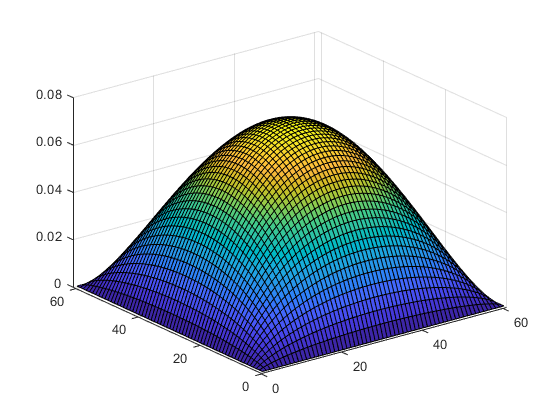
\includegraphics[width=\textwidth]{FIG/MTLB_blocks.png}
			\caption{Solution on square domain}
		\end{figure}
	\end{column}
\end{columns}

\end{frame}

\begin{frame}
\frametitle{Weak scaling}

\begin{columns}
	\begin{column}{0.5\textwidth}
		\begin{figure}
			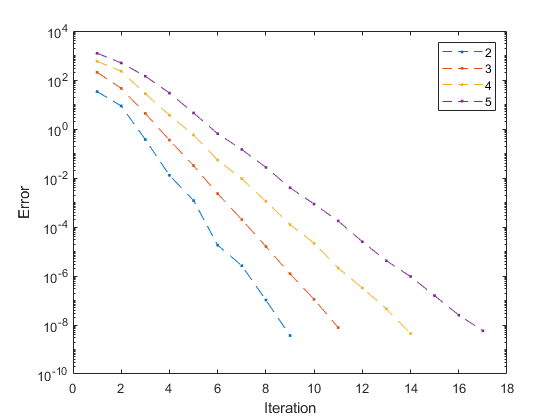
\includegraphics[width=\textwidth]{FIG/MTLB_blocks_weak_error.png}
			\caption{Error in global reconstruction}
		\end{figure}
	\end{column}
	\begin{column}{0.5\textwidth}
		\begin{figure}
			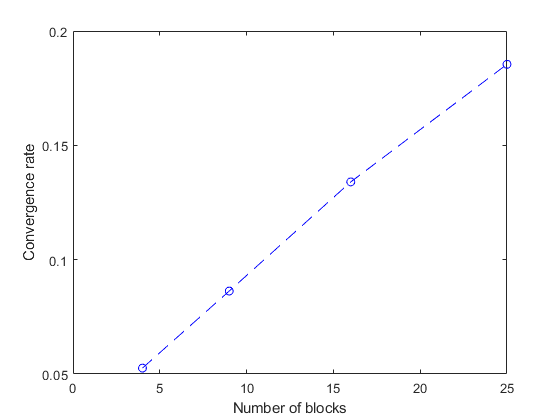
\includegraphics[width=\textwidth]{FIG/MTLB_blocks_weak_conv.png}
			\caption{Convergence rate by number of blocks}
		\end{figure}
	\end{column}
\end{columns}

\end{frame}

\begin{frame}
\frametitle{Strong scaling}

\begin{columns}
	\begin{column}{0.5\textwidth}
		\begin{figure}
			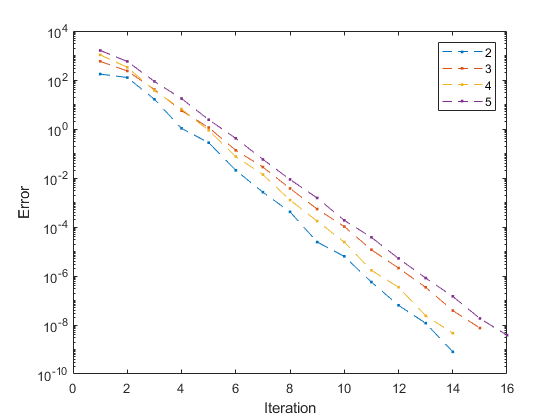
\includegraphics[width=\textwidth]{FIG/MTLB_blocks_strong_error.png}
			\caption{Error in global reconstruction}
		\end{figure}
	\end{column}
	\begin{column}{0.5\textwidth}
		\begin{figure}
			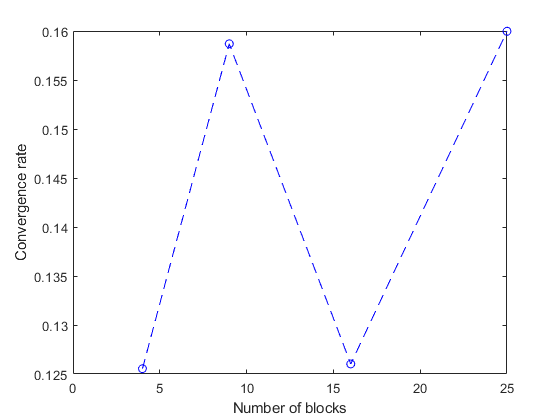
\includegraphics[width=\textwidth]{FIG/MTLB_blocks_strong_conv.png}
			\caption{Convergence rate by number of blocks}
		\end{figure}
	\end{column}
\end{columns}

\end{frame}

\begin{frame}
\frametitle{Conclusions and future work}

\begin{itemize}
\item Symmetrized cells is a highly parallelizable method for constructing highly convergent transmission matrices
\item Global reconstruction is scalable for some simple, small examples
\item Scalability needs to be tested on HPC examples with a parallelized code base
\end{itemize}

\end{frame}

\end{document}